\documentclass{exam}
\usepackage[exos]{main}

\title{Propriétés de fonction}
\date{5 Avril 2024}
\author{Seconde 9}
\pagestyle{empty}

\begin{document}
\maketitle
\thispagestyle{empty}
\begin{minipage}{0.45\textwidth}
\begin{questions}
\question Pour chacune des fonctions suivantes, tracer la courbe représentative sur calculatrice ou sur Geogebra, puis donner son tableau de variation.
\begin{parts}
\part $\function{f}{\left[0;3\right]}{\R}{x}{x^2-5x+1}$ 
\part $\function{g}{\left[1;5\right]}{\R}{x}{\dfrac{1}{x}-2x}$
\part $\function{h}{\left[-3;3\right]}{\R}{x}{x^3+2}$
\end{parts}
\question Les tableaux de variations suivants sont-ils cohérents ? Justifier.

\vspace*{0.2cm}
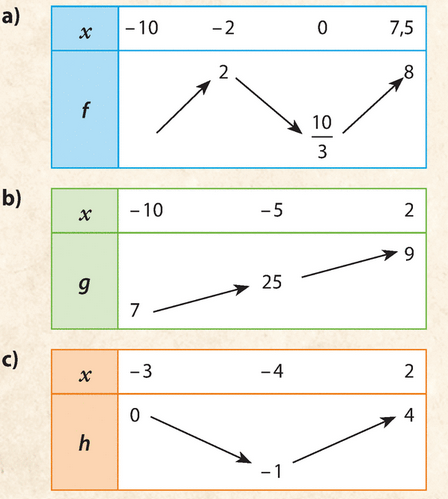
\includegraphics[width=0.9\textwidth]{Exo2.png}
\question
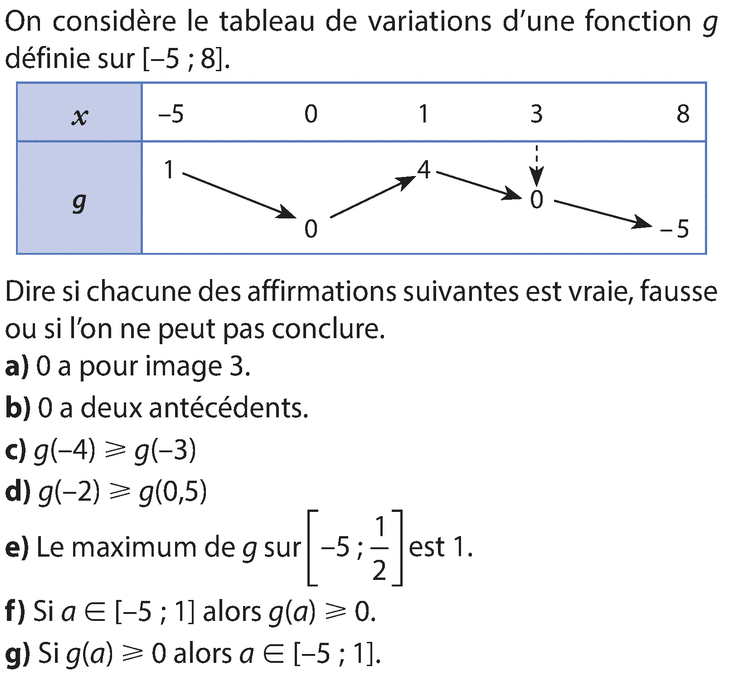
\includegraphics[width=0.9\textwidth]{Exo5.png}
\end{questions}
\end{minipage}
\hfill
\begin{minipage}{0.45\textwidth}
\begin{questions}
\question Pour chacune des fonctions suivantes, tracer la courbe représentative sur calculatrice ou sur Geogebra, puis donner son tableau de variation.
\begin{parts}
\part $\function{f}{\left[-1;2\right]}{\R}{x}{4x^3-5x+2,5}$ 
\part $\function{g}{\left[0;6\right]}{\R}{x}{\dfrac{3x-6}{x+2}}$
\part $\function{h}{\left[-2;2\right]}{\R}{x}{x^4-2x^2}$
\end{parts}
\question
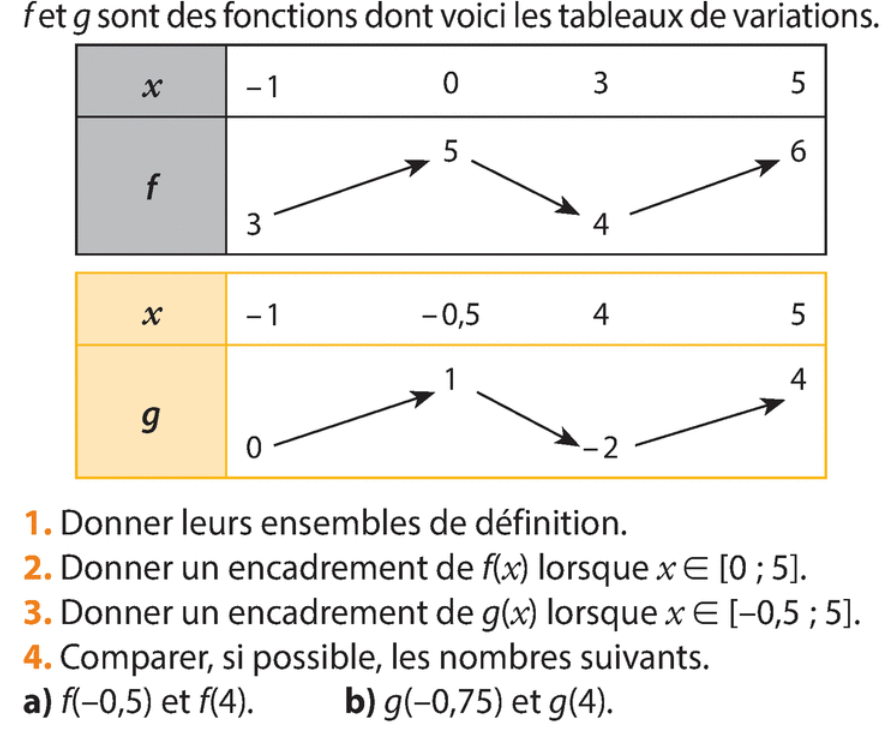
\includegraphics[width=0.9\textwidth]{Exo4.png}
\question
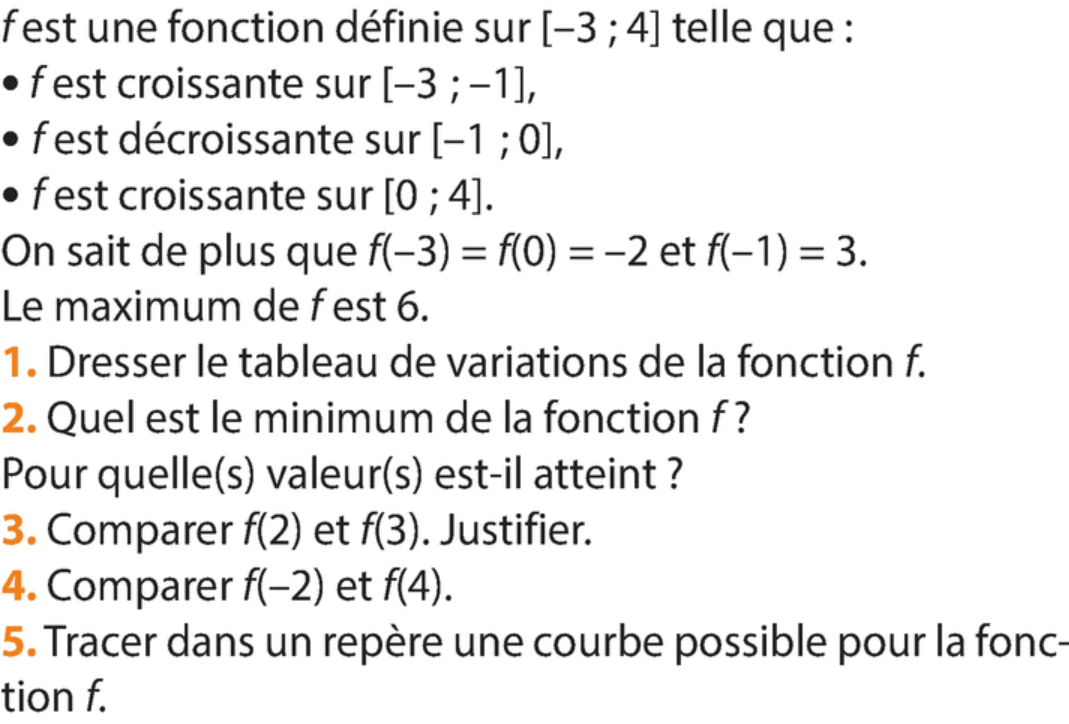
\includegraphics[width=0.9\textwidth]{Exo3.png}
\end{questions}
\end{minipage}
\newpage
\paragraph{Exercice 4}
\begin{center}
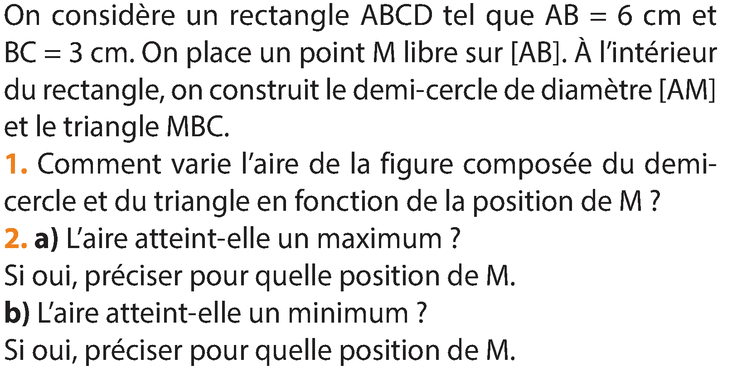
\includegraphics{Exo6.png}
\end{center}
\end{document}